\documentclass{beamer}%Beamer is a LaTeX document class for creating slides for presentations.
\usetheme{metropolis}%


\usepackage{graphicx}%this package allows graphics inclusion
\usepackage{subcaption}
\usepackage[utf8]{inputenc}
\usepackage[spanish, mexico]{babel} %specify document language
%\usepackage[usenames, dvipsnames]{color}

\definecolor{pur}{RGB}{139,0,139}
\definecolor{ver}{RGB}{46,139,87}


\title{Base de Datos Avanzada}%Course name
\date{\today}%Can be set to a specific date with "2018 Agosto 08". "\date" must be used before "\maketitle"
\author{Edher Nu\~no \\ Miguel Ochoa} % \\ breaks the line
\institute{Universidad Aut\'onoma de Guadalajara}


\begin{document}
\maketitle %render title page

\section{Problem\'atica}

\begin{frame}{Problema}
Colecci\'on de peliculas con :
\begin{itemize}
\item Entradas repetidas sin control.
\item Pocas a nulas referencias para intercambio.
	\begin{itemize}	%on beamer "\subitem" can't be used, this is an alternative
		\item[a)] Estudio.
		\item[b)] Director.
	\end{itemize}	
\item Informaci\'on de parametros.
	\begin{itemize}
		\item[a)] Duraci\'on.
		\item[b)] Budget vs Revenue.
	\end{itemize}		
\end{itemize}
\end{frame}

\section{Dise\~no de la base de datos.}
\begin{frame}{Diagrama Entidad-Relaci\'on}
\centering
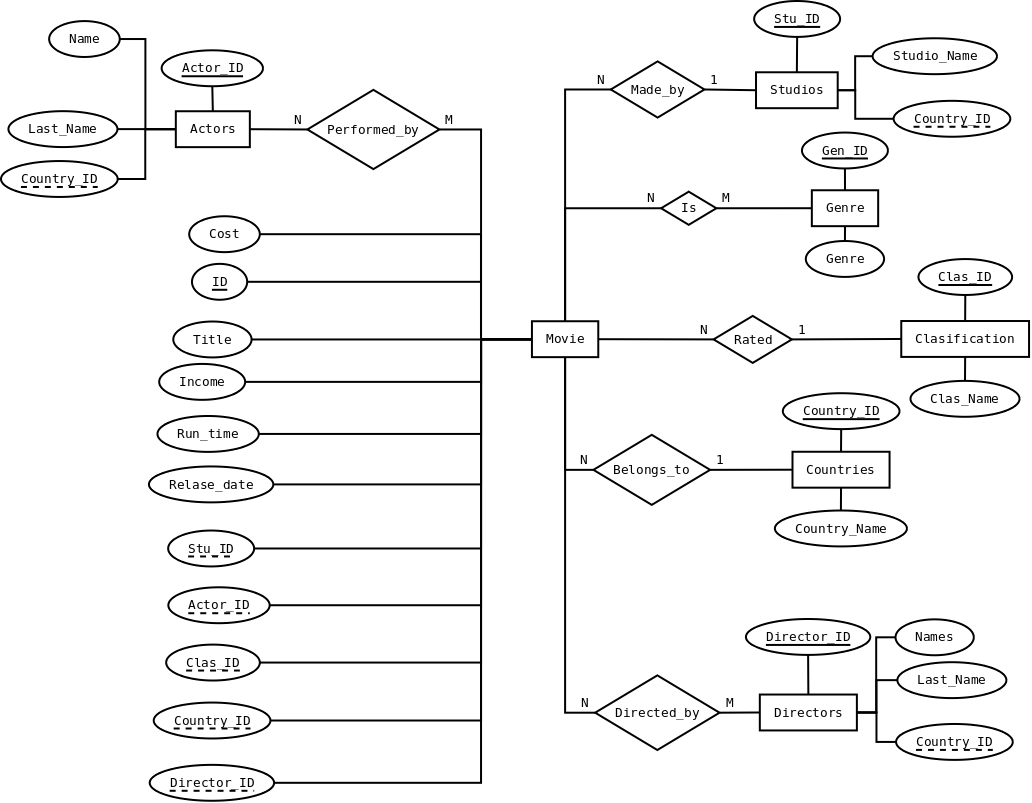
\includegraphics[scale=0.295]{figures/entidad_relacion_01.png}
\end{frame}

\section{Implementaci\'on}
\begin{frame}{Implementaci\'on}
\centering
\begin{tabular}{p{4cm}cp{4cm}}
\texttt{\textcolor{pur}{CREATE TABLE} COUNTRY (ID \textcolor{ver}{INTEGER} \textcolor{pur}{NOT NULL} GENERATED ALWAYS AS IDENTITY (START WITH 1 INCREMENT BY 1), NAME \textcolor{ver}{VARCHAR(30)} \textcolor{pur}{UNIQUE NOT NULL},
    PRIMARY KEY(ID)
);}

& \hspace{1cm} &
 Crea la tabla de paises con el campo ID como llave primaria y generada autom\'aticamente\\
\end{tabular}
\end{frame}

\begin{frame}{Implementaci\'on}
db2 LIST TABLES FOR SCHEMA MOVIEINDEX
\begin{center}
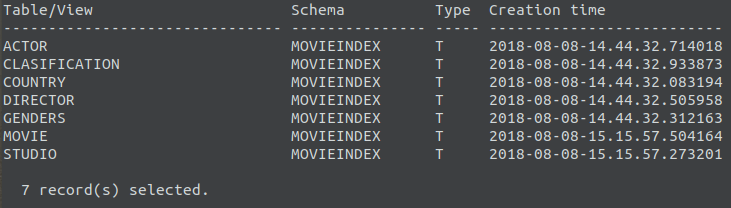
\includegraphics[scale=0.4]{figures/screenshot_output_list_tables.png}
\end{center}
\end{frame}

\begin{frame}{Implementaci\'on}
db2 DESCRIBE TABLE MOVIEINDEX.MOVIE
\begin{center}
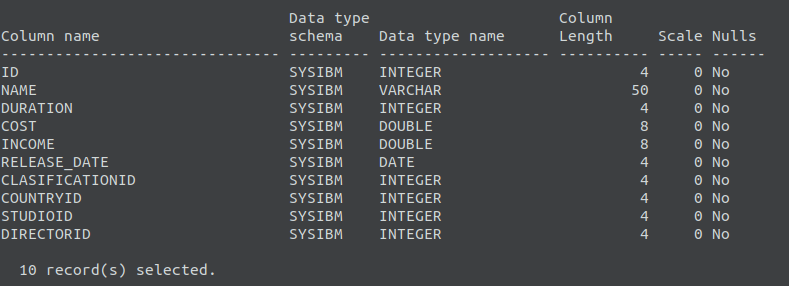
\includegraphics[scale=0.4]{figures/screenshot_output_movie_description.png}
\end{center}
\end{frame}


\begin{frame}{Tablas}
\begin{figure}
    \centering
    \begin{subfigure}[b]{0.3\textwidth}
        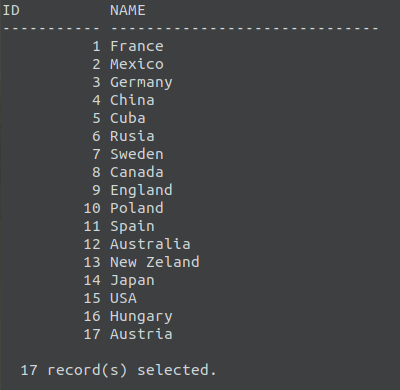
\includegraphics[scale=0.2]{figures/screenshot_country_data.png}
        \caption{Country Table}

    \end{subfigure}
    ~ %add desired spacing between images, e. g. ~, \quad, \qquad, \hfill etc. 
      %(or a blank line to force the subfigure onto a new line)
    \begin{subfigure}[b]{0.4\textwidth}
        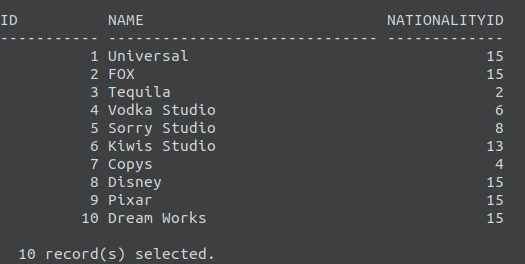
\includegraphics[scale=0.2]{figures/screenshot_studio_data.png}
        \caption{Studio Table}

    \end{subfigure}
    ~ %add desired spacing between images, e. g. ~, \quad, \qquad, \hfill etc. 
    %(or a blank line to force the subfigure onto a new line)
    \begin{subfigure}[b]{0.3\textwidth}
        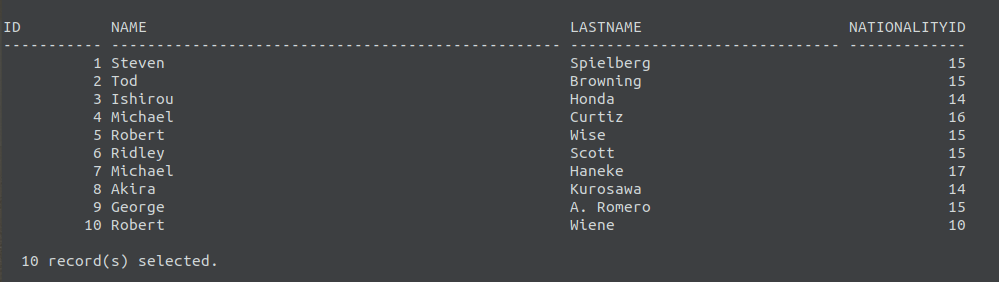
\includegraphics[scale=0.2]{figures/screenshot_director_data.png}
        \caption{Director Table}

    \end{subfigure}
    \caption{Tablas en la MOVIESDB parte 1}
\end{figure}
\end{frame}

\begin{frame}{Tablas}
\begin{figure}
    \centering
    \begin{subfigure}[b]{0.3\textwidth}
        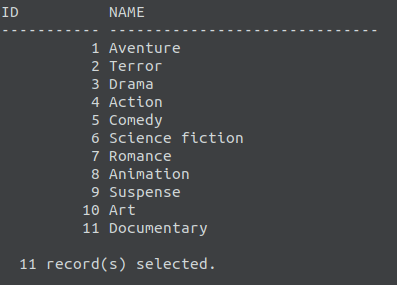
\includegraphics[scale=0.2]{figures/screenshot_gender_data.png}
        \caption{Gender Table}

    \end{subfigure}
    ~ %add desired spacing between images, e. g. ~, \quad, \qquad, \hfill etc. 
      %(or a blank line to force the subfigure onto a new line)
    \begin{subfigure}[b]{0.4\textwidth}
        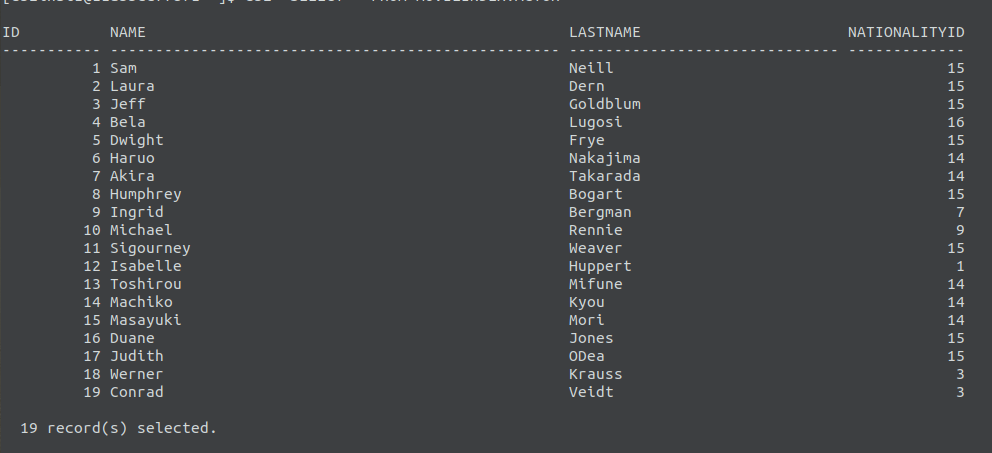
\includegraphics[scale=0.2]{figures/screenshot_actor_data.png}
        \caption{Actor Table}

    \end{subfigure}
    ~ %add desired spacing between images, e. g. ~, \quad, \qquad, \hfill etc. 
    %(or a blank line to force the subfigure onto a new line)
    \begin{subfigure}[b]{0.3\textwidth}
        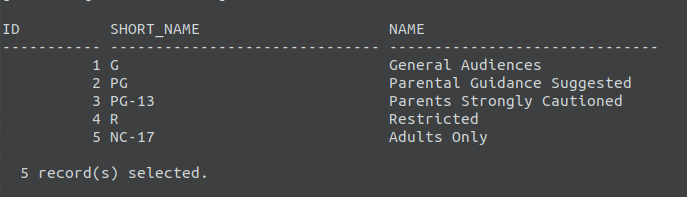
\includegraphics[scale=0.2]{figures/screenshot_clasification_data.png}
        \caption{Clasification Table}

    \end{subfigure}
    \caption{Tablas en la MOVIESDB parte 2}
\end{figure}
\end{frame}


\end{document}
 